\documentclass{article}
\usepackage{amsmath}
\usepackage{graphicx}
\usepackage{listings}
\usepackage{xcolor}
\usepackage{amsmath}
\usepackage{amssymb}
\usepackage{hyperref}
\usepackage{graphicx}
\usepackage{tikz}
\usepackage{geometry}
\usepackage{tcolorbox}
\geometry{margin=0.6in} % margins (default is ~1.5-1.75in)
\usetikzlibrary{positioning}

\usepackage{xcolor} % for dark mdoe
% \definecolor{dark}{HTML}{1F1F1F}
% \pagecolor{dark}
% \color[rgb]{1,1,1}

%%% >>> MY INFORMATION >>>
%%% Name: Kiarash Sotoudeh
%%% Student ID: 1010052194
%%% Email: kiarash.sotoudeh@mail.utoronto.ca
%%% <<< MY INFORMATION <<<

\definecolor{navyblue}{rgb}{0.0, 0.0, 0.5}
\definecolor{myblue}{RGB}{20, 80, 220}
\definecolor{answer}{RGB}{0, 20, 180}


\title{CSC311: Assignment 1 Writeup}
\author{Kiarash Sotoudeh}
\date{} 

% custom colors for code elements
\definecolor{codekeyword}{rgb}{0.0, 0.0, 0.6}
\definecolor{codecomment}{rgb}{0.0, 0.5, 0.0}
\definecolor{codestring}{rgb}{0.6, 0.0, 0.0}

% the listings package
\lstset{
  language=C,                      % language C  
  basicstyle=\ttfamily\small,      % font type and size
  keywordstyle=\color{codekeyword}\bfseries, % keyword color and style
  commentstyle=\color{codecomment}\itshape,  % comment color and style
  stringstyle=\color{codestring},  % string literal color
  numbers=left,                    % line numbers on the left
  numberstyle=\tiny\color{gray},   % line number style
  frame=single,                    % a frame around the code
  breaklines=true,                 % line breaking
  backgroundcolor=\color{white},   % background color
  tabsize=4,                       % tab size
  showspaces=false,                
  showstringspaces=false           
}

\begin{document}

\maketitle

\section*{Question 1}
\subsection*{(a)} 
Suppose we have a classification dataset where each data point has one feature. The feature takes on a real value between $[0, 1]$. What is the minimum number of data points we need to guarantee that any new test point is within ($\leq$) $0.01$ of an old point? (equivalently: What is the smallest set of points S such that every point in $[0,1]$ is within 0.01 of a point in S?) \\
\color{answer}
\textbf{Answer: 50 points.} \\
We want every point in $[0, 1]$ to be within max $0.01$ of a point in $S$. We can divide the interval $[0, 1]$ into intervals of length $0.02$. This is because in worst case scenario, the new test point is in the middle of two existing points and in that case the distance to the nearest point is $0.01$. The example set of points is $S = \{0.01, 0.03, 0.05, \ldots, 0.99\}$. Counting these points we see that only 50 points are needed. \\ 
\color{black}

% % visualization
% \begin{center}
%     \begin{tikzpicture}[scale=10]
%         % draw the interval
%         \draw[->] (0,0) -- (1.02,0) node[right] {x};
%         \draw (0,0) node[below] {0} (1,0) node[below] {1};
%         % plot points at 0.01,0.03,...,0.99
%         \foreach \i in {1,3,...,99} {
%             \fill (\i/100,0) circle[radius=0.003];
%         }
%     \end{tikzpicture}
% \end{center}

\subsection*{(b)}
Explain why such a guarantee is more difficult to maintain when we are working on a problem with $10$ features. \\
\color{answer}
\textbf{Answer:}
When we have 10 features we have to make sure the new test point is within $0.01$ of an old point in all 10 dimensions. In that case we have to check the distance for each component of the vector. According to the curse of dimensionality discussed during class, the total volume of $[0, 1]^d$ is 1 and so $O((\frac{1}{\epsilon})^d)$ points are needed to cover the space. This means for $d=10$ with $\epsilon=0.01$ we need $O((\frac{1}{0.01})^{10}) = O(10^{20})$ points to cover the space! 
\color{black}
\subsection*{(c)}
For each choice of dimension $d \in [2^0, 2^1, 2^2, \dots, 2^{10}]$, sample 100 points from the unit cube, and record the following average distances between all pairs of points, as well as the standard deviation of the distances.
\begin{itemize}
    \item (i) Squared Euclidean or $\ell_2$ distance = $\| \mathbf{x} - \mathbf{y} \|_2^2 = \sum_j (x_j - y_j)^2$
    \item (ii) $\ell_1$ distance = $\| \mathbf{x} - \mathbf{y} \|_1 = \sum_j |x_j - y_j|$
\end{itemize}
Plot both the average and standard deviation as a function of d. \\
\color{answer}
\textbf{Answer:}
\begin{figure}[h!]
    \centering
    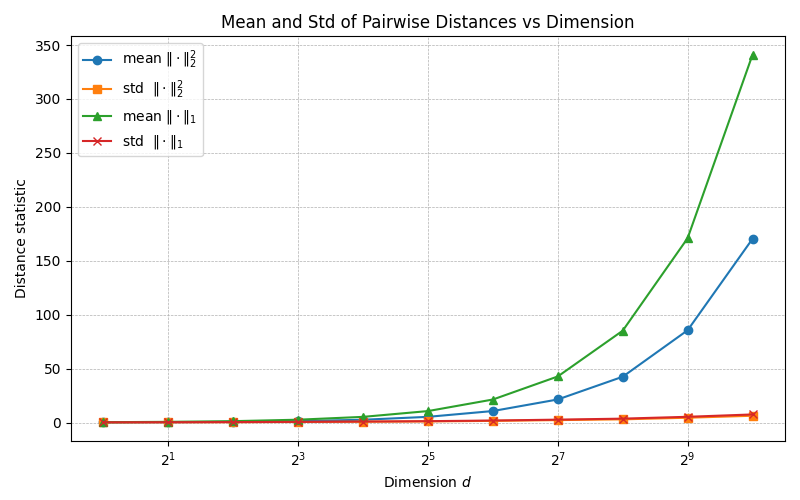
\includegraphics[width=0.5\textwidth]{images/Figure_1_combined.png}
    \caption{Average and standard deviation of distances for $\ell_2$ and $\ell_1$ distances.}
    \label{fig:distances}
\end{figure}

\color{black}
\subsection*{(d)}
Define the squared Euclidean distance $R = Z_1 + \cdots + Z_d$ with $Z_i = (X_i - Y_i)^2$. Given that:
\begin{center}
$\mathbb{E}[Z_i] = \frac{1}{3} \quad \text{and} \quad \mathrm{Var}[Z_i] = \frac{20}{23}$
\end{center}
determine $\mathbb{E}[R]$ and $\mathrm{Var}[R]$ using the properties of expectation and variance. You may give your answer in terms of the dimension $d$. \\
\color{answer}
\textbf{Answer:} Since each coordinate of $\mathbf{X}$ and $\mathbf{Y}$ is sampled independently from the uniform distribution on $[0,1]$ meaning it is $\sim \mathrm{Uniform}[0,1]$, we can use the property given to us to calculate the answer.
\begin{itemize}
    \item $\mathbb{E}[R] = \mathbb{E}[Z_1 + Z_2 + \cdots + Z_d] = \mathbb{E}[Z_1] + \mathbb{E}[Z_2] + \cdots + \mathbb{E}[Z_d] = d \cdot \frac{1}{3} = \frac{d}{3}$
    \item $\mathrm{Var}[R] = \mathrm{Var}[Z_1 + Z_2 + \cdots + Z_d] = \mathrm{Var}[Z_1] + \mathrm{Var}[Z_2] + \cdots + \mathrm{Var}[Z_d] = d \cdot \frac{20}{23} = \frac{20d}{23}$
\end{itemize}
\color{black}
\subsection*{(e)}
In probability theory, one can derive that
$\mathbb{P}(|Z - \mathbb{E}[Z]| \geq a) \leq \frac{\mathrm{Var}[Z]}{a^2}
$for any random variable Z. (This fact is known as Markov’s Inequality.) Based on your answer to part (d), explain why does this support the claim that in high dimensions, “most points are approximately the same distance”? Let’s justify this step-by-step: \\\\
(i) We want to bound the probability that any given distance R is at least r away from its expectation. Define E as the event “R is at least r away from its expectation”. How would you write E in mathematical notation? \\\\
\color{answer}
\textbf{Answer:} \\
$ E \;=\;\bigl\lvert R - \mathbb{E}[R]\bigr\rvert \;\ge\; r. $ \\\\
\color{black}
(ii) Use Markov’s Inequality to bound $\mathbb{P}(E)$. \\\\
\color{answer}
\textbf{Answer:} \\
We already calculate din part (d) that we have
$\mathbb{E}[R]=\tfrac d3$ and $\mathrm{Var}[R]=\tfrac{20}{23}\,d$. So plugging them into the given inequality we get $\mathbb{P}(E)
=\mathbb{P}\bigl(|R-\mathbb{E}[R]|\ge r\bigr)
\;\le\; \frac{\,\tfrac{20}{23}\,d\,}{r^{2}}$ \space or \space $\mathbb{P}(E)=\mathbb{P}\bigl(|R-\frac{d}{3}|\ge r\bigr) \;\le\; \frac{\,\tfrac{20}{23}\,d\,}{r^{2}}$\\\\
\color{black}
(iii) Let r in part (i) be proportional to distance (and therefore dimension), i.e. r = cd. Apply the result in part (ii) and note what happens to $\mathbb{P}(E)$ as d goes to $\infty$. \\\\
\color{answer}
\textbf{Answer:} \\
We plug in $r=cd$ into the inequality we just got in part (ii) and we get: \\
$\mathbb{P}(E)=\mathbb{P}\bigl(|R-\frac{d}{3}|\ge cd\bigr) \;\le\; \frac{\,\tfrac{20}{23}\,d\,}{(cd)^{2}}=\frac{20}{23c^{2}d}$ \\
Since we have one $d$ in the denominator, as $d$ goes to $\infty$, the probability $\mathbb{P}(E)$ goes to $0$. Intuitively, this means that as the dimension increases, the probability of a point being far away from the mean distance decreases which supports what we've seen in the previous parts of the assignment. So in high dimensions, most distances between pairs of points are close to their mean, so most points are around the same distance from each other.\\
\color{black}
\section*{Question 2}
\subsection*{(a)}

\end{document}
